\section{The \sys System}\label{s:arch}
 
\begin{figure}[t]
\centering
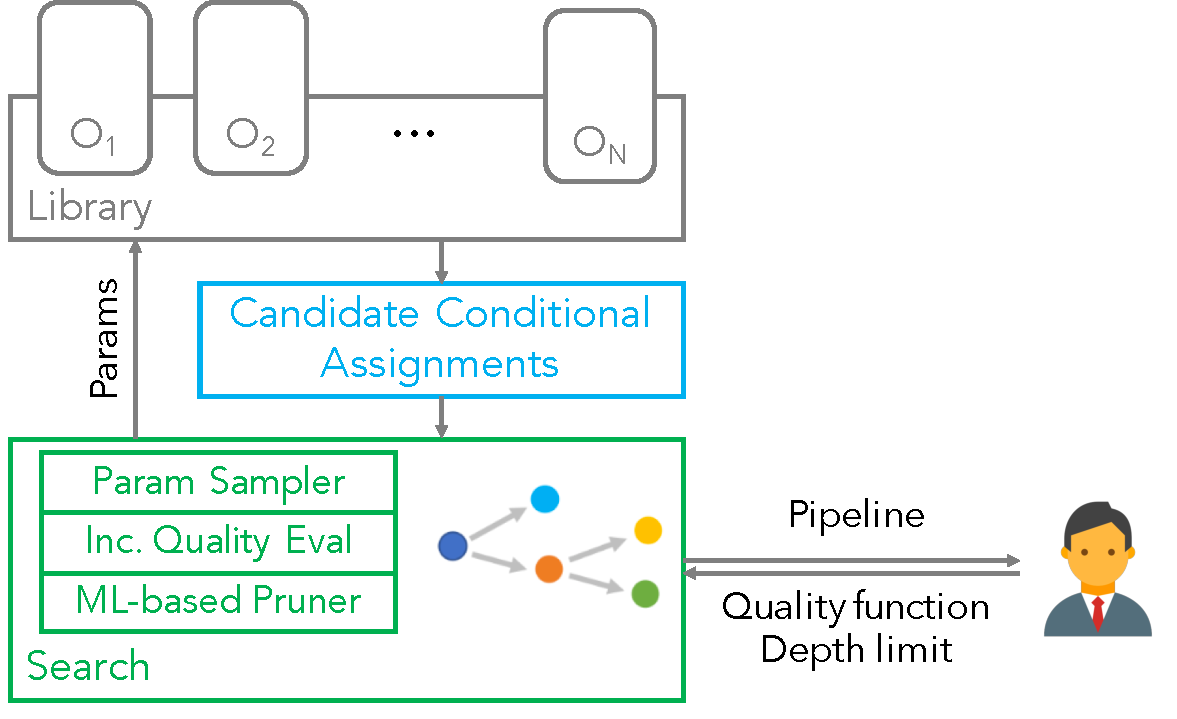
\includegraphics[width=\columnwidth]{figures/arch.pdf}
\caption{\sys system architecture.}
\label{f:arch}
\end{figure}

Figure~\ref{f:arch} depicts the primary components of the system architecture. The \blue{blue} component manages the detection and repair libraries while the \orange{orange} components execute the Boost-and-Clean algorithm to generate the sequence of conditional repairs $\mathcal{L}^*$.  To generate $\mathcal{L}^*$, \sys takes as input training and test datasets, where the only restriction is that the test labels are correct. 

\sys first executes the library of detector generators on the training dataset to produce a set of candidate predicates (Section~\ref{s:detectorgen}).    The {\it Boost-and-Clean} component takes these predicates, along with the repair functions, as input and selects a subset of the pairs (conditional repairs).  To do so, it iteratively selects the next conditional repair by appending it to the sequence of repairs so far, training a new classifier using the sequence and evaluating it using the {\it Test Accuracy Evaluator}.  We also call this process {\it repair selection}.  Finally, the conditional repairs $\mathcal{L}^*$ are sent to the {\it Deployer}, which compiles the sequence into a  classifier that can detect and repair errors in the test records so that the predictions are robust to the detected data errors.  

\sys is pre-populated with a library of detector generators and repair functions that work well in practice (Section~\ref{s:exp}).  However,  developers can also specify custom detection or repair functions that fit their domain.  To further simplify how the system can be used, developers can implement familiar feature extraction functions, and the {\it IsoDetect} component will automatically translate them into detector generator functions.

\subsection{Detectors}
The ability for a data cleaning system to accurately identify data errors relies on the availability of a set of high-quality error detection rules~\cite{DBLP:conf/sigmod/ChuIKW16}.  To help developers easily implement new detector generators, we have implemented \detectlib, a library that transforms feature extraction functions into detector generators automatically.  Also, to help developers quickly bootstrap their data cleaning process, \sys includes a pre-populated library of simple feature extraction functions that are effective at detecting data errors across a wide range of domains and data science applications (Section~\ref{s:exp}).  We note that these libraries are not meant to replace domain knowledge, but rather to address routine problems.

\subsubsection{The \detectlib Library}
Although developers may directly implement detector generators as described in Section~\ref{s:detectorgen}, we found that many cleaning detection algorithms in machine learning workflows, including \company, follow a fixed outlier-detection structure: first they convert a record into a feature vector,  select threshold(s) over one or more features in the vector such that if the thresholds are exceeded, then the record is identified as a candidate dirty record.  Although developers often have a clear sense of useful features to extract from the dataset, it is often unclear how to tune the thresholds and for which features thresholds should be defined for.  

For this reason, \detectlib employs a modular approach that automatically performs the latter threshold tuning task so that developers can focus on feature engineering.   Developers simply define featurization functions that map records into a numerical feature vector; for each featurizer, \detectlib executes it and performs outlier detection to select the combination of features and thresholds that will identify the outliers.  

We considered a number of outlier detection algorithms to use.  A recently popular approach is a robust estimator of the sample population variance called Minimum Covariance Determinant~\cite{rousseeuw2011robust} (MCD), which has been used in systems such as MacroBase~\cite{bailis2016macrobase}.  The key limitation is that the technique is computationally expensive and can have degenerate results (due to rank-deficient covariance matrices).

We instead use a variant of Random Forest classification, called Isolation Forests~\cite{liu2008isolation}.  The Isolation Forest is inspired by the observation that outliers are more easily separable from the rest of the dataset than non-outliers.  It grows a forest of isolation trees, where each tree is randomly grown---it selects a random attribute and a random threshold value---until a leaf node contains a single record.  The length of the path to the leaf node is a measure for the outlier-ness of the record---a shorter path more strongly suggests that the record is an outlier.  The isolation forest creates a large set of isolation trees and classifies records with short average path length as outliers.  In contrast to computational expensive algorithms such as MCD, Isolation Forests have a linear time complexity and very small memory requirements.  

A nice property of the technique is that the resulting forest can be simplified and efficiently compiled into simple threshold rules. 
For example, if a featurizer extracts a scalar feature in $\mathbb{R}$ (e.g., $n\_emp$), the Isolation Forest will generate a single-attribute threshold rule (e.g., $n\_emp > 2$).  
 We experimented with alternative outlier detection techniques (e.g., Minimum Covariance Determinant) but found that the Isolation Forest provided the best trade-off between runtime and accuracy.
 
\stitle{Hyper-parameters: } The Isolation Forest has a few hyper-parameters that need to be tuned, namely, the maximum branch length and a threshold that determines outlier v.s. not outlier. As much as possible, we have tuned these hyper-parameters generically with sensible defaults. Experimentally, we find that performance does not suffer too much with the default parameters.
In one of our experiments, we used a single hyper-parameter setting across all datasets and evaluate accuracy. 
 
\stitle{False Positive and False Negatives: } In general, a predicate learned from data will have false positives and false negatives.
This is why the boosting selection is important.
If a predicate is too uncertain and applies the repair to many spurious records, then it will reduce classification accuracy.
By boosting, we can protect the system against uncertain detectors.

\subsubsection{Pre-populated Featurizers}
\noindent We have implemented four classes of featurizers:

\stitle{Numerical Attributes: } This featurizer projects the numerical attributes into a feature vector.  We find that this is effective at identifying numerical outliers that are statistically different from the rest of the data. For example, the sensor dataset has sensor readings on the order of $300C$ when typical readings are $17C$ (Section \ref{exp:comp}).

\stitle{Missing Values: }  We manually enumerated a set of regular expression patterns that commonly describe missing values in a database.  These include \textsf{NULL} attribute values; patterns such as empty string, NaN, Inf; or values whose string representations lack alphanumeric characters. Each pattern corresponds to a boolean feature in the extracted feature vector.   Although this is a hand-curated list, it is easily extensible and is effective at identifying missing values. 11 out of the 13 experimental datasets, had some form of missing value error.

\stitle{Parsing/Type Errors: } We use each attribute's type signature to check whether an attribute value matches the type signature.  For numerical attributes, the featurizer outputs whether the entry can be parsed into a floating point number or an integer. For dates and address types, we check whether common components (e.g., Month, Day, Year for dates, Street, City for addresses) are found using common date and address parsing libraries.   This means that the entry has a minimum of the required components (Month, Day, Year) or (Street, City, State).  This is implemented with standard python libraries: \textsf{usaddress} and \textsf{datetime}. The FEC dataset had a small number of rows with the wrong number of columns, leading to data type errors. 
We have a ``short-circuit'' routine for featurizers to declare an attribute an instant failure without passing it into \detectlib.

\stitle{Text Errors using Word Embeddings: }
Although the above featurizers are effective for quantitative attributes, many datasets contain string-valued and categorial attributes that are not amenable to the above approaches.  Also, naively featurizing text attributes using, e.g., hot-one encoding, can easily increase the dimensionality of the dataset to tens of thousands or millions of dimensions---even a two-attribute relation with one numerical and one string-valued attribute, may have thousands of features.  The statistical power of outlier detection techniques rapidly diminishes in the high-dimensional feature-spaces.

In response, we borrow the recent concept of text embeddings from Natural Language Processing to featurize record values into a lower-dimensional vector-space.  
Text embeddings are models trained on a corpus of documents that embed words from the corpus into a vector-space where nearby vectors are similar words.
This allows one to featurize string and categorical values into numerical vectors, and evaluate similarity relationships between documents in this vector-space.

We adapt the popular \textsf{word2vec} model~\cite{mikolov2013distributed} to structured outlier detection. 
We treat each record as a document, where each attribute value is a ``word''. 
The model learns to embed attributes that co-occur in the same records closer in the vector-space.
Thus, each attribute value is mapped to a vector, and each record is the concatenation of its attributes' vectors.  
The isolation forest then takes this vector as input to generate an appropriate predicate.  

The isolation forest has the crucial property that the anomaly detection criteria are axis-aligned cuts.  Since each set of features corresponds to a record attribute, we can directly translate threshold violations into the data attributes that are erroneous.
In our experiments, we find that this approach is effective at detecting a variety of categorical errors that we did not explicitly code for.
One common example is when a header record (i.e., one specifying the names all the attributes) is included in the dataset.
The model identifies this record as containing values not typically present in the dataset.
Similarly, this module detected oddly formatted codes in the FEC dataset.

\subsubsection{Adding Custom Featurizers} 
Our featurizers are meant to be a starting point that is supplemented by domain specific modules. For example, if the data scientist knows that employee ids in a database must match a particular pattern, she can build featurizers to parse these ids. Similarly, if the data scientist knows something about the structure of the features (e.g., they are time-series), she can add in other features such as frequency components derived from an FFT. All of these featurizers must return a vector and a mapping between vector components and base-data attributes.


\iffalse
    \subsection{Loader}
    The first step in using \sys is loading a dataset. \sys requires that that data is initially weakly structured, similar to the assumptions of SQLShare~\cite{howe2013sqlshare}. It assumes that each row corresponds to a record and attributes are delimited, but there are potentially missing values, the domain of possible attribute values are unknown, and the data types are unknown.
    We implemented a schema-on-read loading module that takes as input a SQL table, CSV, or a text file.
    This module returns a structured relation of tuples and inferred data types for each attribute (numerical, categorical, string, date, address).
    We designed the type inference to be soft--allowing for errors to exist in the dataset.
    The module automatically builds indices over the numerical and categorical attributes.
    These indices will help optimize the error detection module.
\fi



\subsection{Repairs}
In addition to detector generators, \sys is pre-populated with a set of simple repair functions.  A function is applied to all records identified by a detector's predicate.  In the following five repair functions, the first three can be used as data and prediction repair functions,  whereas the fourth is for data repair, and the last is for prediction repair:

\stitle{Mean Imputation (data and prediction): } Impute a cell in violation with the mean value of the attribute calculated over the training data excluding violated cells.


\stitle{Median Imputation (data and prediction): } Impute a cell in violation with the median value of the attribute calculated over the training data excluding violated cells.

\stitle{Mode Imputation (data and prediction): } Impute a cell in violation with the most frequent value of the attribute calculated over the training data excluding violated cells.  In contrast to mean and median imputation, this is also applicable to non-numerical attributes.

\stitle{Discard Record (data): } Discard a dirty record from the training dataset.  This restriction to only training data is to ensure that a degenerate solution---simply deleting all test data---is disallowed. 

\stitle{Default Prediction (prediction): } Automatically predict the most popular label from the training dataset for a row that matches the conditional repair's predicate.

% The cleaner's role is to learn an assignment of these actions to each of the violations.  The combination of the actions and the predicates define the data cleaning libary $\mathcal{L}$.



\subsection{Optimizations}
In order to borrow the error bound guarantees, the Boost-and-Clean algorithm (Algorithm~\ref{s:boostalg}) is a direct translation of AdaBoost and a naive implementation of the algorithm can be expensive.  Namely, it takes as input the cross product of predicates and repair function and, in each iteration, requires applying the conditional repairs, and training and testing a classifier for each conditional repair.  
To reduce the cost, we employ optimizations to address three bottlenecks in the naive algorithm.  These optimizations are developed specifically to speed up the Boost-and-Clean repair selection process, and we did not attempt to optimize the detection nor data parsing and loading steps of the end-to-end system.  For the purposes of this paper, we additionally assume that the test datasets fit into memory (the training data do not have this restriction).

\stitle{Prediction Materialization: } Our first observation is that the cleaning operations actions do not change between iterations of the boosting algorithm--only the weights for computing the accuracy change.  Thus, we pre-train the classifiers $C_i$ corresponding to each conditional repair $l_i$, and materialize their predictions on the test records $C_i(X_{test})$.  

\stitle{Prediction Indexing: } Computing the score for each classifier requires retrieving the the weights of the test records that are mis-predicted and correctly predicted.  We speed up these lookups using a hash index for each classifier that that maps prediction labels to their corresponding test records.
%the weights of the records , for each $j$ in the output domain of the classifier $C$, stores the mapping $j \mapsto \{x : C_i(x) == j \wedge x \in X_{test}\}$.

\stitle{Parallelization: }  Finally, many of the operations in Boost-and-Clean, such as classifier training and scoring, must be performed for each conditional repair.  We create and execute a thread for each conditional repair to perform each task in parallel.  We leave more advanced optimization techniques such as within-training parallelization~\cite{recht2011hogwild} and sampling the training data for future work.